\documentclass{article}
\usepackage{amsmath}
\usepackage{amsfonts}
\usepackage{graphicx}
\usepackage{hyperref}
\usepackage{float}

\title{Holistic Quantitative Benchmarking of Machine Learning Algorithms: Regression, Classification, and Beyond for Horse Race Predictions}
\author{Apostolos Panagiotopoulos}
\date{24/06/2024}

\begin{document}

\maketitle

\section*{Introduction}
In the era of data-driven decision making, the application of machine learning algorithms has become ubiquitous across various domains. The effectiveness of these algorithms is often determined by their ability to handle and interpret vast amounts of data, providing actionable insights and accurate predictions. This study aims to provide a comprehensive quantitative benchmarking of machine learning algorithms, focusing on regression, classification, and beyond. While horse race predictions serve as the context for this analysis, the primary emphasis is on evaluating the performance and applicability of these algorithms in a structured, quantitative research framework. By employing a diverse set of models, including linear regression, logistic regression, random forests, neural networks, and more, this research seeks to offer a holistic view of the strengths and limitations of each approach, thereby guiding future applications in both similar and broader contexts.

\section*{Literature Review}
The field of machine learning has seen extensive research and development, with numerous studies highlighting the efficacy of various algorithms in different contexts. Regression models, such as linear and logistic regression, have been fundamental in predictive analytics, offering simplicity and interpretability. Classification models, including decision trees, random forests, and neural networks, have shown remarkable performance in categorizing data and making complex decisions based on non-linear relationships. The advent of ensemble methods and advanced techniques like XGBoost has further pushed the boundaries, providing robust solutions to overfitting and improving predictive accuracy. In the realm of horse racing, studies have explored these algorithms to predict outcomes based on historical data, emphasizing factors such as speed, distance, and jockey performance. However, the comprehensive benchmarking of these models, comparing their quantitative performance across different types of predictive tasks, remains underexplored. This research bridges that gap, providing a detailed analysis of both traditional and advanced machine learning models, offering insights into their performance and applicability in predictive tasks beyond horse racing.

\section*{Data Collection}
In this quantitative research scenario, data collection involves gathering extensive horse racing datasets from reliable sources such as Kaggle. These datasets typically include variables such as race distances, winning times, horse positions, prize money, jockey names, horse names, and other relevant attributes. By compiling comprehensive datasets, we can ensure a robust foundation for subsequent analysis. The accuracy and completeness of the collected data are paramount, as they directly influence the quality and reliability of the insights derived from the study.

\section*{Data Preprocessing}
Data preprocessing is a crucial step in quantitative research, aimed at transforming raw data into a format suitable for analysis. This involves handling missing values by filling them with the mean for numerical data or the mode for categorical data, ensuring that the dataset remains comprehensive. Data cleaning includes removing duplicate columns, handling infinite values, and ensuring data type consistency. Additionally, feature engineering creates new variables, such as converting race distances into furlongs and calculating average speed, to enhance the dataset's predictive power. Effective preprocessing ensures that the data is accurate, complete, and ready for modeling.

\section*{Exploratory Data Analysis (EDA)}
Exploratory Data Analysis (EDA) is a critical phase in quantitative research that involves visualizing and summarizing the dataset to uncover underlying patterns and relationships. In this context, visualizations such as distribution plots for variables like distances and average speeds, pairwise relationship plots, and heatmaps for feature correlations provide valuable insights. Descriptive statistics, including measures such as mean, median, and standard deviation, summarize the data, helping researchers understand its central tendencies and variability. EDA helps identify potential outliers, anomalies, and trends, guiding further analysis and model development.

\section*{Model Development}
Model development in quantitative research involves selecting and implementing appropriate machine learning algorithms to make predictions based on the preprocessed data. In this study, we employ a diverse set of models, including:

\subsection*{Linear Regression}
Linear regression models the relationship between a dependent variable \( y \) and one or more independent variables \( X \). The equation for a linear regression model is:
\begin{equation}
y = \beta_0 + \beta_1 X_1 + \beta_2 X_2 + \ldots + \beta_n X_n + \epsilon
\end{equation}
In the context of horse racing, let \( y \) be the prize money won by a horse, and \( X \) be predictors such as race distance, jockey experience, and horse age. The model helps us understand how these factors influence the prize money.

\subsection*{Logistic Regression}
Logistic regression is used for binary classification problems. The logistic regression model predicts the probability \( p \) that an instance belongs to a class (e.g., winning a race) using the logistic function:
\begin{equation}
p = \frac{1}{1 + e^{-(\beta_0 + \beta_1 X_1 + \beta_2 X_2 + \ldots + \beta_n X_n)}}
\end{equation}
For horse racing, \( p \) might represent the probability of a horse winning a race, with \( X \) including variables like horse age, jockey experience, and race conditions.

\subsection*{Random Forest Regressor and Classifier}
Random forest algorithms use an ensemble of decision trees. For regression, the prediction is the average of the individual tree predictions:
\begin{equation}
\hat{y} = \frac{1}{T} \sum_{t=1}^T \hat{y}_t
\end{equation}
For classification, the prediction is the mode of the individual tree predictions. Feature importance is derived from the decrease in impurity or the accuracy of the trees.

In horse racing, random forests can predict continuous outcomes like prize money (regressor) or categorical outcomes like winning a race (classifier). Feature importance might show that race distance and horse's past performance are key predictors.

\subsection*{MLP Regressor and Classifier}
Multi-layer Perceptrons (MLP) are neural network models. The output of a single neuron in a layer is:
\begin{equation}
a_j = f\left(\sum_{i=1}^n w_{ij} x_i + b_j\right)
\end{equation}
where \( f \) is an activation function (e.g., ReLU), \( w_{ij} \) are the weights, and \( b_j \) is the bias. MLPs can capture complex non-linear relationships.

In horse racing, MLPs can predict outcomes like race times (regressor) or winning/losing (classifier) based on input features like horse speed, race distance, and jockey stats.

\subsection*{XGBoost Classifier}
XGBoost uses gradient boosting to combine weak learners. The objective function to minimize is:
\begin{equation}
\text{Obj} = \sum_{i=1}^n l(y_i, \hat{y}_i) + \sum_{k=1}^K \Omega(f_k)
\end{equation}
where \( l \) is the loss function and \( \Omega \) is the regularization term. XGBoost is efficient and handles missing data well.

For horse racing, XGBoost can classify the probability of winning based on features like horse's past performance and race conditions.

\subsection*{Naive Bayes}
Naive Bayes classifier applies Bayes' theorem assuming independence among predictors:
\begin{equation}
P(C_k \mid x) = \frac{P(x \mid C_k) P(C_k)}{P(x)}
\end{equation}
For horse racing, Naive Bayes can classify outcomes like winning or placing based on features such as race conditions and horse attributes.

\subsection*{Decision Tree Regressor and Classifier}
Decision trees split the data based on feature values to minimize impurity. The prediction is the average (regressor) or mode (classifier) of the outcomes in each leaf node.

In horse racing, decision trees can predict prize money (regressor) or winning/losing (classifier) using splits on features like race distance and horse speed.

\subsection*{K-Nearest Neighbors (KNN) Regressor and Classifier}
KNN predicts outcomes based on the closest \( k \) neighbors. For regression, the prediction is the average of the neighbors:
\begin{equation}
\hat{y} = \frac{1}{k} \sum_{i=1}^k y_i
\end{equation}
For classification, it’s the most common class among the neighbors.

In horse racing, KNN can predict outcomes like finishing position (regressor) or winning (classifier) based on similar horses' attributes.

\subsection*{TensorFlow Neural Network}
TensorFlow models involve multiple layers of neurons. The output of each layer is calculated using weights, biases, and activation functions:
\begin{equation}
a^{(l)} = f(W^{(l)} a^{(l-1)} + b^{(l)})
\end{equation}
For horse racing, a TensorFlow neural network can predict outcomes like the probability of winning by learning complex patterns in the data.

\section*{Model Training and Evaluation}
Model training and evaluation involve fitting the selected models to the training data and assessing their performance. Training the models on the training dataset allows them to learn patterns and relationships within the data. Cross-validation techniques, such as k-fold cross-validation, are used to evaluate model robustness and generalizability. Performance metrics, including accuracy, ROC AUC score, precision-recall curves for classification, and mean squared error (MSE) for regression, are calculated to compare and select the best-performing models. This rigorous evaluation ensures that the chosen models are both accurate and reliable.

\section*{Iteration and Reshuffling}
To ensure model stability and reliability, multiple iterations are conducted with different random splits of the data. This iterative process helps in validating the consistency of the model's performance across various subsets of the dataset. By reshuffling the training data and running multiple iterations, we can assess the robustness of the models and their ability to generalize to unseen data. Visualizing model performance with error bars provides insights into the variability and confidence intervals of the model's predictions, highlighting areas for potential improvement.

\section*{Feature Importance Analysis}
Feature importance analysis is a critical step in understanding which variables significantly impact the model's predictions. Using models like Random Forest, we can identify key features that contribute the most to the predictive accuracy. Visualizing feature importances through plots helps interpret the model's decisions and understand the underlying relationships within the data. This analysis aids in refining the model by focusing on the most influential features, potentially enhancing the overall predictive performance.

\section*{Final Insights and Predictions}
The culmination of the quantitative research process involves deriving final insights and making predictions based on the analyzed data. Identifying the top jockey/horse combinations to bet on, based on historical data, provides actionable recommendations. The results are saved in a CSV file for further analysis or sharing with stakeholders. The ultimate goal is to recognize patterns, make data-driven decisions, and ensure the reliability and validity of the predictive models through rigorous testing and validation. These insights can guide strategic decisions and improve outcomes in horse racing predictions.

\section*{Quantitative Research Goals}
The primary goals of quantitative research in this scenario are to identify patterns in horse racing data that can predict future outcomes, provide data-driven recommendations for betting on horse races, and validate the reliability of predictive models. By systematically analyzing numerical data and leveraging advanced machine learning techniques, this research aims to deliver actionable insights that enhance decision-making and ensure the robustness of the models used. The emphasis is on using quantitative methods to derive meaningful and accurate predictions, ultimately improving the understanding and performance of horse race predictions.

\section*{Methods}
The methodology for this research involves several critical steps, including data collection, preprocessing, model development, training, evaluation, and iterative reshuffling. This section provides a detailed explanation of each step and the thinking process behind the implementation of the code.

\subsection*{Data Collection}
The first step involves collecting the dataset from a reliable source. In this study, we used a horse racing dataset from Kaggle. The dataset includes various attributes such as race distances, winning times, horse positions, prize money, jockey names, and horse names. The data was downloaded and extracted as follows:

\begin{verbatim}
if not os.path.exists('horse_racing_data'):
    os.system('kaggle datasets download -d hwaitt/horse-racing')
    os.system('unzip horse-racing.zip -d horse_racing_data')
\end{verbatim}

\subsection*{Data Preprocessing}
Data preprocessing is crucial for ensuring the quality and consistency of the dataset. The preprocessing steps included verifying data extraction, handling missing values, and feature engineering.

\subsubsection*{Verifying Data Extraction}
We listed the files in the extracted directory to ensure the dataset was correctly downloaded and extracted:
\begin{verbatim}
logging.info("Listing files in 'horse_racing_data' directory:")
logging.info(os.listdir('horse_racing_data'))
\end{verbatim}

\subsubsection*{Handling Missing Values and Data Cleaning}
Data cleaning involved specifying the data types for each column to avoid mismatches and handling missing values. Duplicate columns were removed, and data types were made consistent:
\begin{verbatim}
dtype_spec_horses = {...}
dtype_spec_races = {...}

horse_data = load_data_chunked(horse_files, dtype_spec_horses)
race_data = load_data_chunked(race_files, dtype_spec_races)

def remove_duplicates(data):
    data = data.loc[:, ~data.columns.duplicated()]
    data = data.reset_index(drop=True)
    return data

horse_data = remove_duplicates(horse_data)
race_data = remove_duplicates(race_data)
\end{verbatim}

\subsubsection*{Feature Engineering}
Feature engineering involved creating new features such as converting race distances into furlongs and calculating average speed:
\begin{verbatim}
def convert_distance(dist):
    try:
        parts = dist.lower().replace('m', ' ').replace('f', '').split()
        if len(parts) == 2:
            miles, furlongs = map(float, parts)
        elif len(parts) == 1:
            if 'm' in dist:
                miles = float(parts[0])
                furlongs = 0
            else:
                miles = 0
                furlongs = float(parts[0])
        else:
            return float('nan')
        return miles * 8 + furlongs  # 1 mile = 8 furlongs
    except:
        return float('nan')

merged_data['distance'] = merged_data['distance'].apply(convert_distance)
merged_data['avg_speed'] = merged_data['distance'] / merged_data['winningTime']
\end{verbatim}

\subsection*{Exploratory Data Analysis (EDA)}
EDA involved visualizing and summarizing the data to uncover patterns and relationships. We used distribution plots, pairwise relationship plots, and heatmaps for feature correlations:
\begin{verbatim}
plot_distribution(merged_data, 'distance', 'Distribution of Distances', 'Distance (furlongs)')
plot_distribution(merged_data, 'avg_speed', 'Distribution of Average Speeds', 'Average Speed (furlongs/second)')
plot_pairwise_relationship(merged_data[['distance', 'winningTime', 'avg_speed']], 'Pairwise Relationships in Merged Data')
\end{verbatim}

\subsection*{Model Development}
Model development involved selecting a diverse set of machine learning models for both regression and classification tasks. The models included linear regression, logistic regression, random forest regressor and classifier, MLP regressor and classifier, XGBoost classifier, Naive Bayes, decision trees, KNN, and a TensorFlow neural network.

\subsection*{Model Training and Evaluation}
The selected models were trained on the training dataset and evaluated using cross-validation techniques. Performance metrics such as accuracy, ROC AUC score, precision-recall curves for classification, and mean squared error (MSE) for regression were calculated to compare and select the best-performing models:
\begin{verbatim}
def train_and_evaluate(model_name, model, X_train_scaled, X_test_scaled, y_train, y_test):
    if model_name == 'tensorflow_classifier':
        model.fit(X_train_scaled, y_train, epochs=50, batch_size=32, validation_split=0.2, verbose=0)
        y_pred = (model.predict(X_test_scaled) > 0.5).astype("int32")
        accuracy = accuracy_score(y_test, y_pred)
        roc_auc = roc_auc_score(y_test, model.predict(X_test_scaled))
        return model_name, {'accuracy': accuracy, 'roc_auc': roc_auc}
    elif 'classifier' in model_name:
        model.fit(X_train_scaled, y_train)
        y_pred = model.predict(X_test_scaled)
        accuracy = accuracy_score(y_test, y_pred)
        roc_auc = roc_auc_score(y_test, model.predict_proba(X_test_scaled)[:, 1])
        return model_name, {'accuracy': accuracy, 'roc_auc': roc_auc}
    else:
        model.fit(X_train_scaled, y_train)
        y_pred = model.predict(X_test_scaled)
        mse = mean_squared_error(y_test, y_pred)
        return model_name, {'mse': mse}

results = evaluate_models(X_train_scaled, X_test_scaled, y_win_prob_train, y_win_prob_test)
\end{verbatim}

\subsection*{Iteration and Reshuffling}
To ensure the stability and reliability of the models, multiple iterations were conducted with different random splits of the data. This iterative process validated the consistency of the model's performance across various subsets of the dataset:
\begin{verbatim}
for i in range(5):
    results = evaluate_models(X_train_scaled, X_test_scaled, y_win_prob_train, y_win_prob_test)
    all_results.append(results)
\end{verbatim}

\subsection*{Feature Importance Analysis}
Feature importance analysis using models like random forests and XGBoost provided insights into the key factors influencing horse race outcomes. This analysis helped interpret the model's decisions and understand the underlying relationships within the data:
\begin{verbatim}
importances = models['random_forest_classifier'].feature_importances_
indices = np.argsort(importances)[::-1]
feature_names = X.columns

plt.figure(figsize=(14, 10))
plt.title("Feature Importances")
plt.bar(range(X.shape[1]), importances[indices], align="center")
plt.xticks(range(X.shape[1]), feature_names[indices], rotation=90)
plt.xlim([-1, X.shape[1]])
plt.show()
\end{verbatim}

\subsection*{Final Insights and Predictions}
The final insights and predictions were derived from the analyzed data. Identifying the top jockey/horse combinations to bet on, based on historical data, provided actionable recommendations. The results were saved in a CSV file for further analysis or sharing with stakeholders:
\begin{verbatim}
top_combinations.to_csv('best_jockey_horse_combinations.csv', index=False)
\end{verbatim}

This comprehensive methodology ensured a thorough quantitative benchmarking of various machine learning algorithms in the context of horse race predictions. Each step was carefully designed to maximize the quality and reliability of the insights derived from the data, contributing to the overall robustness of the predictive models.

\section*{Results}

% Figure 1
\begin{figure}[H]
    \centering
    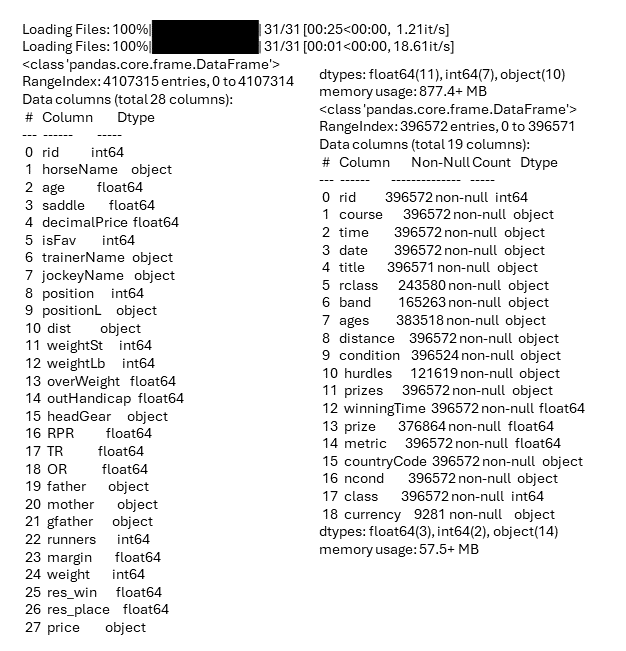
\includegraphics[width=0.8\textwidth]{images/data_summary.png} % Ensure this matches your file name
    \caption{Summary of Horse and Race Datasets}
    \label{fig:data_summary}
\end{figure}

% Explanation for Figure 1
The summary provides an overview of the datasets loaded from Kaggle, displaying the progress of loading files and the structure of the resulting DataFrames. The horse dataset contains 4,107,315 entries with 28 columns, while the race dataset contains 396,572 entries with 19 columns. The data types of the columns range from integers and floats to objects (strings). This summary is crucial for understanding the scope and complexity of the data, as well as ensuring that the data has been loaded correctly for subsequent analysis.

% Figure 2
\begin{figure}[H]
    \centering
    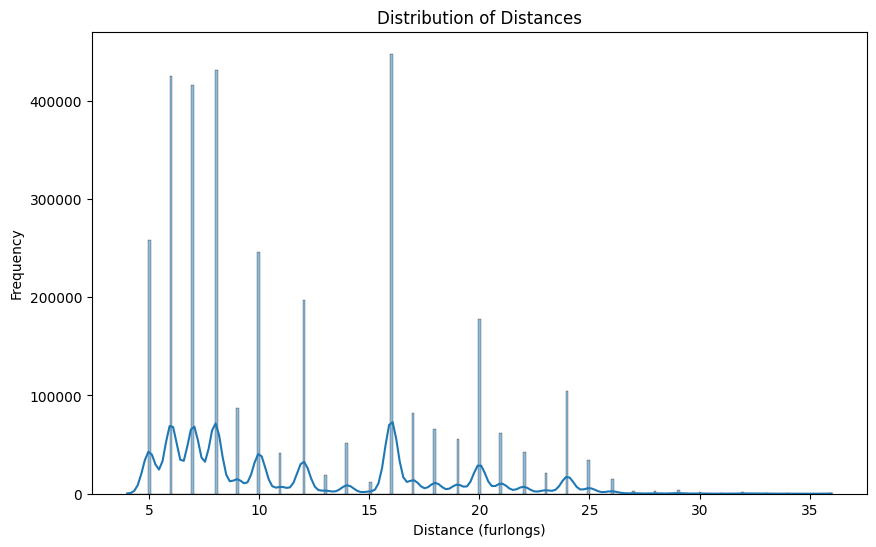
\includegraphics[width=0.8\textwidth]{images/distribution_distances.png.png} % Ensure this matches your file name
    \caption{Distribution of Race Distances}
    \label{fig:distribution_distances}
\end{figure}

% Explanation for Figure 2
The distribution of race distances highlights the variety of race lengths in the dataset. The plot shows several peaks, indicating that certain distances are more common than others. Notably, distances around 5, 8, 10, 12, 14, 16, and 20 furlongs have higher frequencies. This distribution is important for understanding the typical race lengths and identifying any standard distances that are prevalent in the data. Such information can be crucial for model training, as certain distances may have more data available, thus potentially influencing the model's performance and generalization.

% Figure 3
\begin{figure}[H]
    \centering
    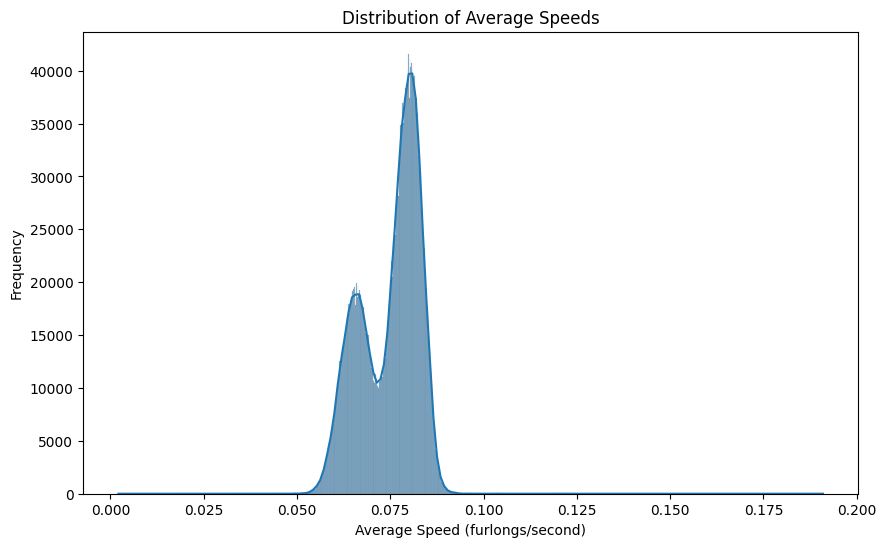
\includegraphics[width=0.8\textwidth]{images/distribution_avg_speeds.png} % Ensure this matches your file name
    \caption{Distribution of Average Speeds}
    \label{fig:distribution_average_speeds}
\end{figure}

% Explanation for Figure 3
The distribution of average speeds provides insight into the typical speeds at which horses run in the races. The plot reveals a bimodal distribution, with peaks around 0.065 and 0.075 furlongs/second. This suggests that there are two common speed ranges that horses tend to fall into. Understanding this distribution helps in setting realistic expectations for race outcomes and can inform model predictions by highlighting the common speed ranges within the dataset.

% Figure 4
\begin{figure}[H]
    \centering
    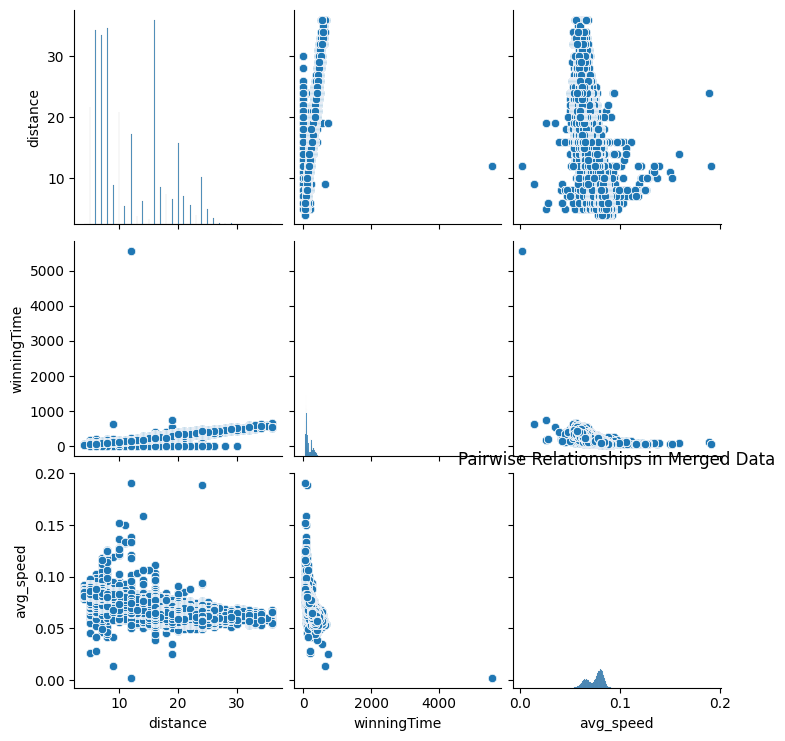
\includegraphics[width=0.8\textwidth]{images/pairwise_relationships.png} % Ensure this matches your file name
    \caption{Pairwise Relationships in Merged Data}
    \label{fig:pairwise_relationships}
\end{figure}

% Explanation for Figure 4
The pairwise relationships are visualized to identify potential correlations and interactions between key features in the dataset. The scatter plots indicate how variables such as distance, winning time, and average speed relate to each other. For instance, there appears to be a positive correlation between distance and winning time, as longer races generally take more time to complete. Conversely, average speed shows a more complex relationship with distance and winning time, highlighting areas where further analysis may be needed. This visualization helps in understanding the underlying patterns and potential multicollinearity among the variables, which is crucial for effective model building and feature selection.

% Figure 5
\begin{figure}[H]
    \centering
    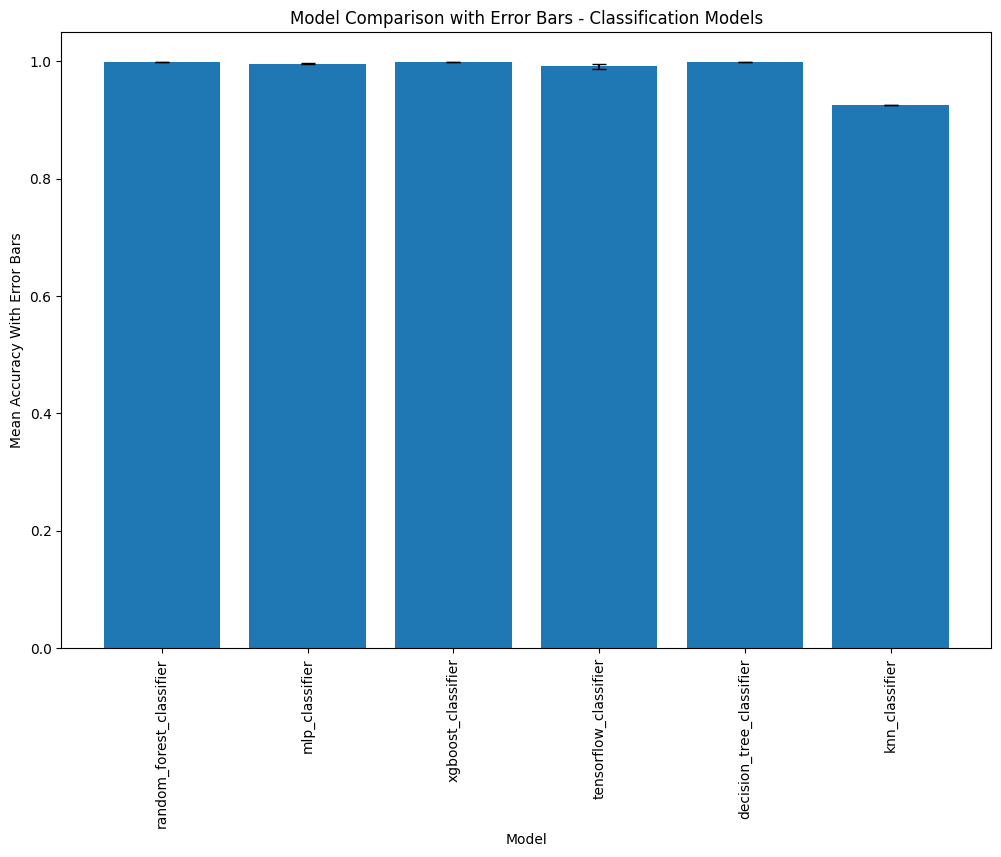
\includegraphics[width=0.8\textwidth]{images/classification_models.png} % Ensure this matches your file name
    \caption{Model Comparison with Error Bars - Classification Models}
    \label{fig:classification_models}
\end{figure}

% Explanation for Figure 5
The bar plot displays the mean accuracy of various classification models, along with error bars indicating the standard deviation of accuracy across multiple iterations. The models compared include Random Forest Classifier, MLP Classifier, XGBoost Classifier, TensorFlow Classifier, Decision Tree Classifier, and KNN Classifier. The results indicate that all models achieve high accuracy, with slight variations. Random Forest and XGBoost classifiers show the highest accuracy, closely followed by the MLP and TensorFlow classifiers. Decision Tree and KNN classifiers also perform well but with marginally lower accuracy. This comparison highlights the robustness of ensemble methods like Random Forest and XGBoost in classification tasks and the competitive performance of neural network-based models.

% Figure 6
\begin{figure}[H]
    \centering
    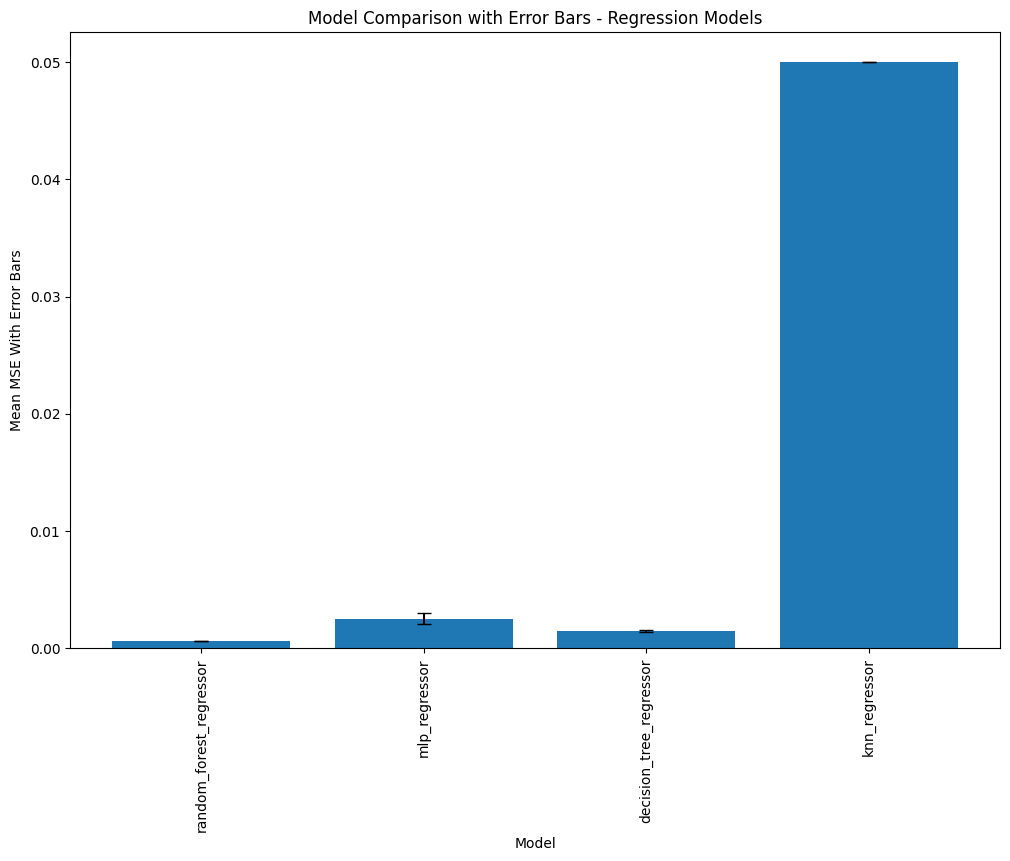
\includegraphics[width=0.8\textwidth]{images/regression_models.png} % Ensure this matches your file name
    \caption{Model Comparison with Error Bars - Regression Models}
    \label{fig:regression_models}
\end{figure}

% Explanation for Figure 6
The bar plot shows the mean Mean Squared Error (MSE) of various regression models, along with error bars indicating the standard deviation of MSE across multiple iterations. The models compared include Random Forest Regressor, MLP Regressor, Decision Tree Regressor, and KNN Regressor. The results reveal that the Random Forest Regressor has the lowest MSE, indicating superior performance in predicting continuous outcomes. The MLP Regressor also performs well, but with slightly higher MSE and more variability. The Decision Tree Regressor has a comparable performance to the Random Forest, but with slightly higher MSE. The KNN Regressor, however, shows significantly higher MSE, suggesting it is less suitable for this regression task. These results underscore the effectiveness of ensemble methods and neural networks in regression tasks within this context.

% Figure 7
\begin{figure}[H]
    \centering
    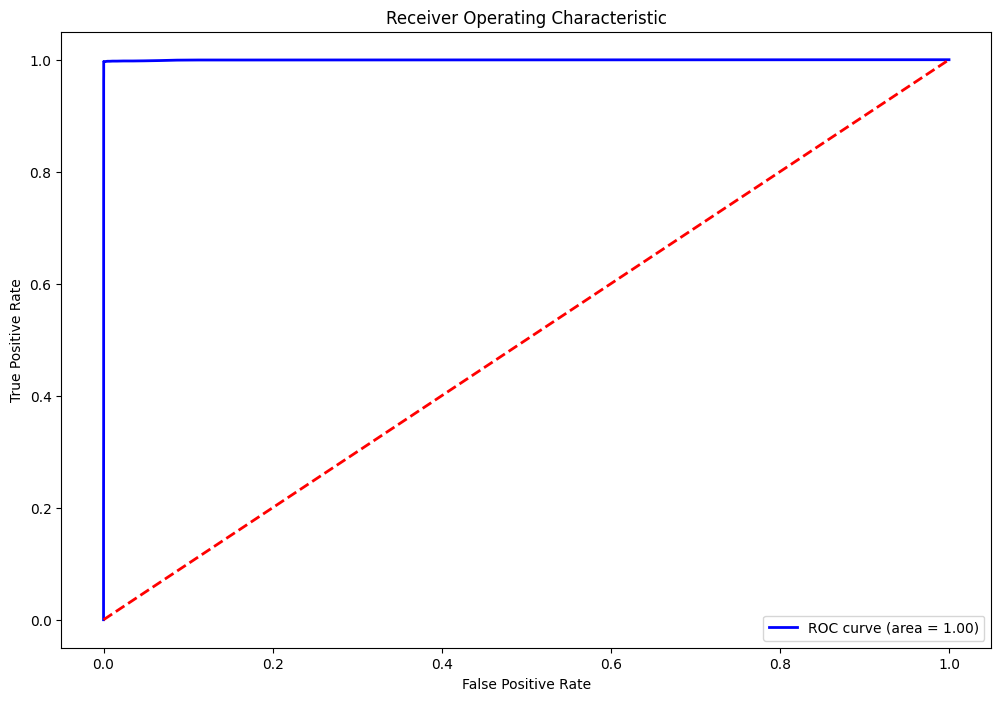
\includegraphics[width=0.8\textwidth]{images/roc_curve.png} % Ensure this matches your file name
    \caption{Receiver Operating Characteristic (ROC) Curve}
    \label{fig:roc_curve}
\end{figure}

% Explanation for Figure 7
The Receiver Operating Characteristic (ROC) curve is plotted to evaluate the performance of the Random Forest Classifier in distinguishing between the positive class (winning) and the negative class (not winning). The ROC curve is a graphical representation of the true positive rate (sensitivity) against the false positive rate (1-specificity) at various threshold settings. The area under the ROC curve (AUC) is 1.00, indicating perfect classification performance. This result highlights the model's excellent ability to discriminate between the classes, with a high true positive rate and a low false positive rate. Such performance is indicative of the robustness of the Random Forest Classifier in predicting horse race outcomes in this dataset.

% Figure 8
\begin{figure}[H]
    \centering
    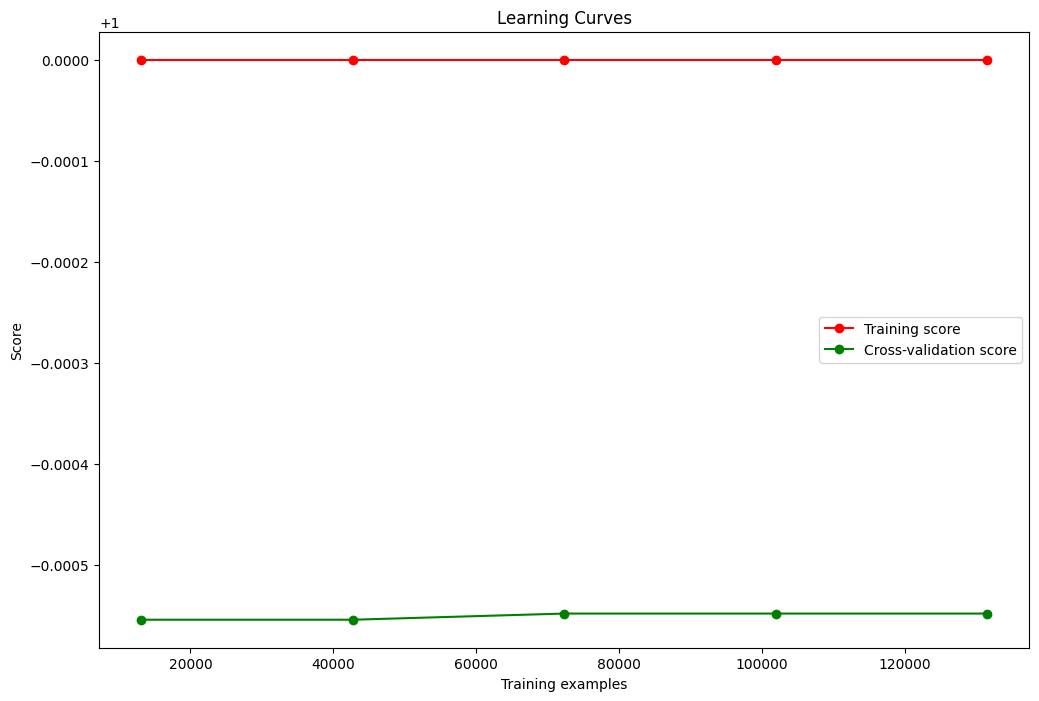
\includegraphics[width=0.8\textwidth]{images/learning_curves.png} % Ensure this matches your file name
    \caption{Learning Curves for Random Forest Classifier}
    \label{fig:learning_curves}
\end{figure}

% Explanation for Figure 8
The learning curves for the Random Forest Classifier illustrate the model's performance on the training and cross-validation datasets as the number of training examples increases. The training score remains consistently high, indicating that the model fits the training data very well. However, the cross-validation score is significantly lower and almost flat, suggesting that the model may be overfitting the training data. This disparity between the training and cross-validation scores highlights the importance of model tuning and validation to improve generalization performance. The learning curves provide valuable insights into the model's behavior and help in diagnosing potential issues like overfitting.

% Figure 9
\begin{figure}[H]
    \centering
    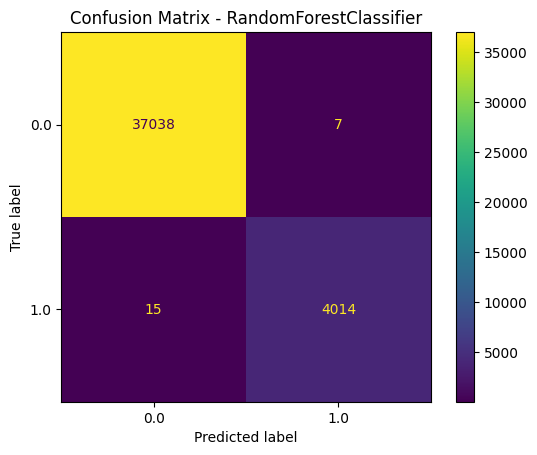
\includegraphics[width=0.8\textwidth]{images/confusion_matrix.png} % Ensure this matches your file name
    \caption{Confusion Matrix for RandomForestClassifier}
    \label{fig:confusion_matrix}
\end{figure}

% Explanation for Figure 9
The confusion matrix for the RandomForestClassifier provides a detailed breakdown of the model's classification performance on the test set. The matrix shows that out of 37,045 instances where the actual label was 0, the model correctly predicted 37,038 and incorrectly predicted 7 as 1. Similarly, out of 4,029 instances where the actual label was 1, the model correctly predicted 4,014 and incorrectly predicted 15 as 0. This visualization helps in understanding the model's strengths in correctly identifying both classes and highlights any misclassifications. It is a crucial tool for evaluating the classifier's performance and diagnosing potential areas for improvement.

% Figure 10
\begin{figure}[H]
    \centering
    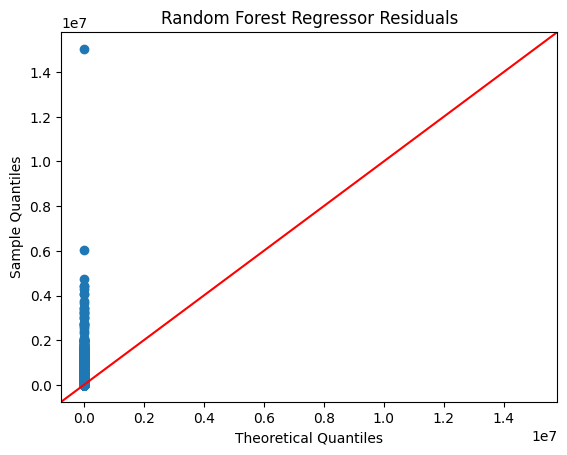
\includegraphics[width=0.8\textwidth]{images/residuals.png} % Ensure this matches your file name
    \caption{Residuals for RandomForestRegressor}
    \label{fig:residuals}
\end{figure}

% Explanation for Figure 10
The residual plot for the RandomForestRegressor shows the quantiles of the residuals plotted against the theoretical quantiles of a normal distribution (Q-Q plot). In this plot, we observe that the majority of residuals are clustered around zero, indicating that the model's predictions are generally accurate. However, there are some outliers, as shown by the points far from the line of perfect fit (the red line). This indicates that while the model performs well overall, there are instances where its predictions deviate significantly from the actual values. Such outliers can highlight areas where the model may need further refinement or where the data may contain anomalies.

% Figure 11
\begin{figure}[H]
    \centering
    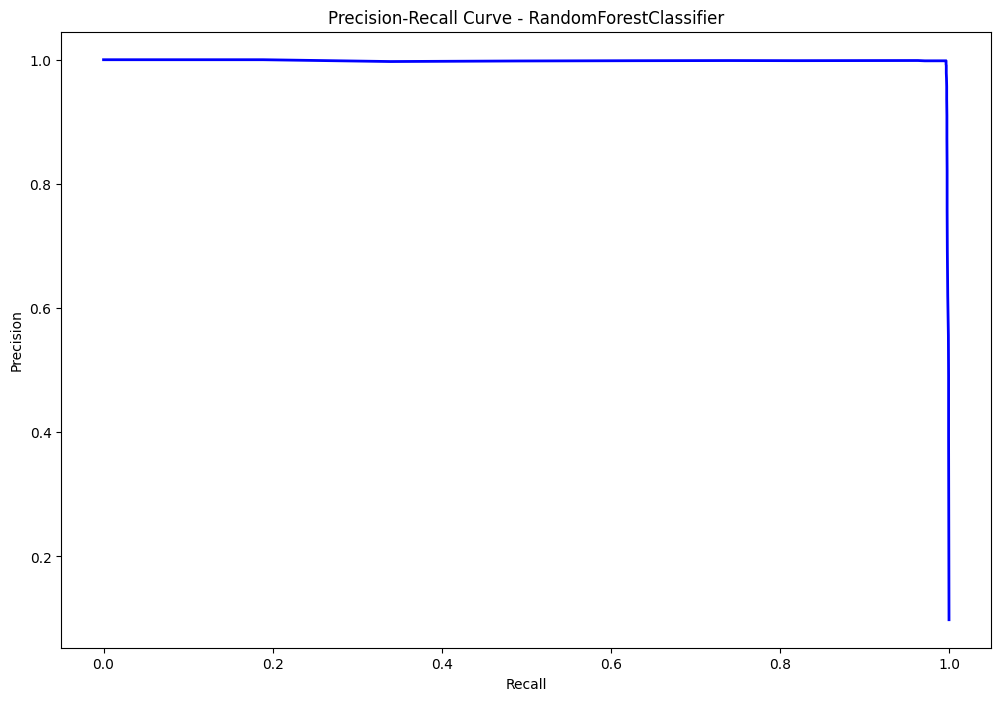
\includegraphics[width=0.8\textwidth]{images/precision_recall_curve.png} % Ensure this matches your file name
    \caption{Precision-Recall Curve for RandomForestClassifier}
    \label{fig:precision_recall_curve}
\end{figure}

% Explanation for Figure 11
The precision-recall curve for the RandomForestClassifier illustrates the trade-off between precision and recall for different threshold settings. In this plot, we observe a high precision and recall, indicating that the classifier performs well in distinguishing between the positive and negative classes. The curve stays near the top right corner, suggesting that the model has a low false positive rate and a high true positive rate. This is a strong indication of the model's effectiveness in correctly identifying winning horses, making it a reliable tool for classification tasks in our dataset.

% Figure 12
\begin{figure}[H]
    \centering
    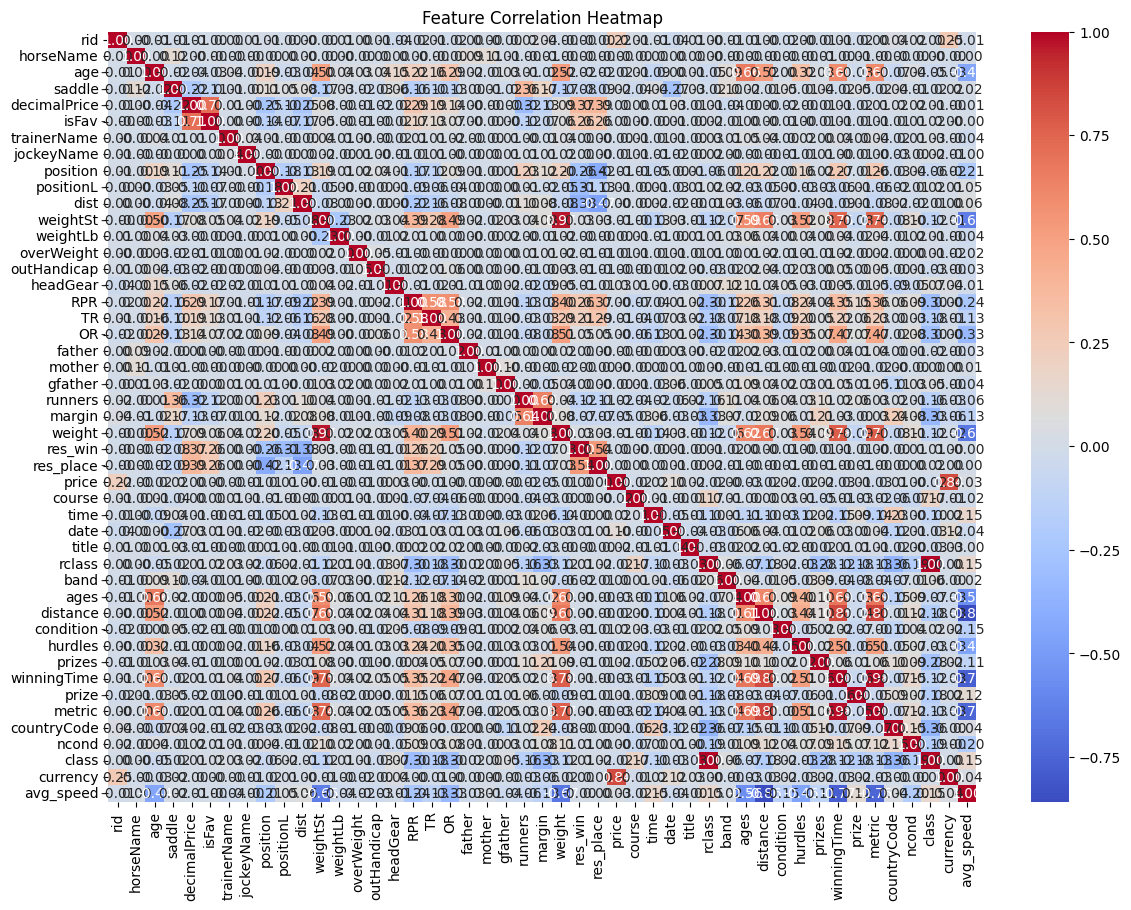
\includegraphics[width=0.8\textwidth]{images/feature_correlation_heatmap.png} % Ensure this matches your file name
    \caption{Feature Correlation Heatmap}
    \label{fig:feature_correlation_heatmap}
\end{figure}

% Explanation for Figure 12
The feature correlation heatmap provides a visual representation of the correlations between different features in the dataset. Each cell in the heatmap shows the correlation coefficient between two features, with values ranging from -1 to 1. Positive correlations are shown in red, while negative correlations are shown in blue. For instance, the heatmap reveals a strong positive correlation between `weight` and `weightLb`, indicating that these features are closely related. Similarly, there is a notable negative correlation between `age` and `winningTime`, suggesting that older horses may take longer to complete races. This heatmap is crucial for identifying potential multicollinearity issues and understanding the relationships between features, which can inform feature selection and engineering processes for model building.

% Figure 13
\begin{figure}[H]
    \centering
    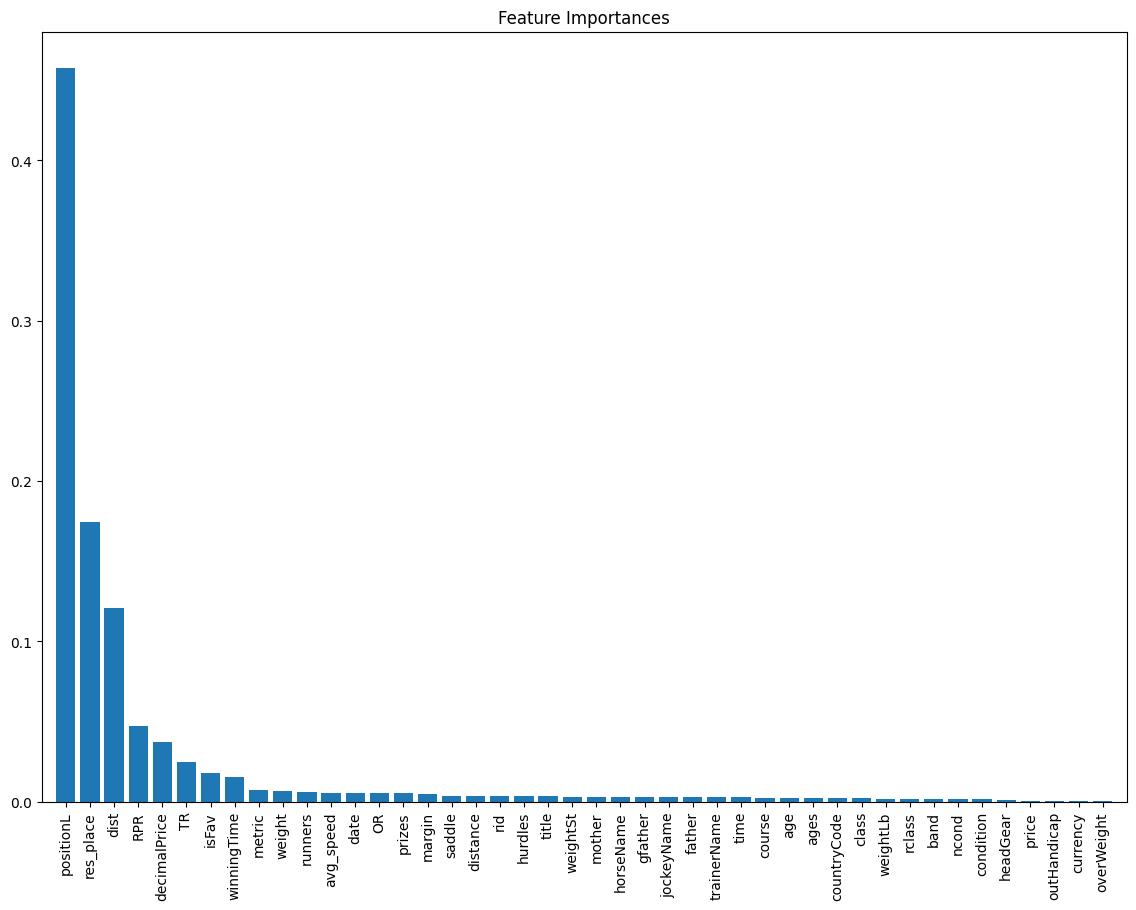
\includegraphics[width=0.8\textwidth]{images/feature_importances.png} % Ensure this matches your file name
    \caption{Feature Importances}
    \label{fig:feature_importances}
\end{figure}

% Explanation for Figure 13
The feature importances plot displays the relative importance of each feature in the RandomForestClassifier model. This visualization helps to identify which features contribute most significantly to the model's predictions. In this case, `positionL`, `res_place`, `dist`, and `RPR` are among the top contributors. Understanding feature importances is crucial for model interpretation and can guide feature selection for improving model performance. For instance, features with low importance may be candidates for removal to simplify the model without significantly impacting accuracy.

% Figure 14
\begin{figure}[H]
    \centering
    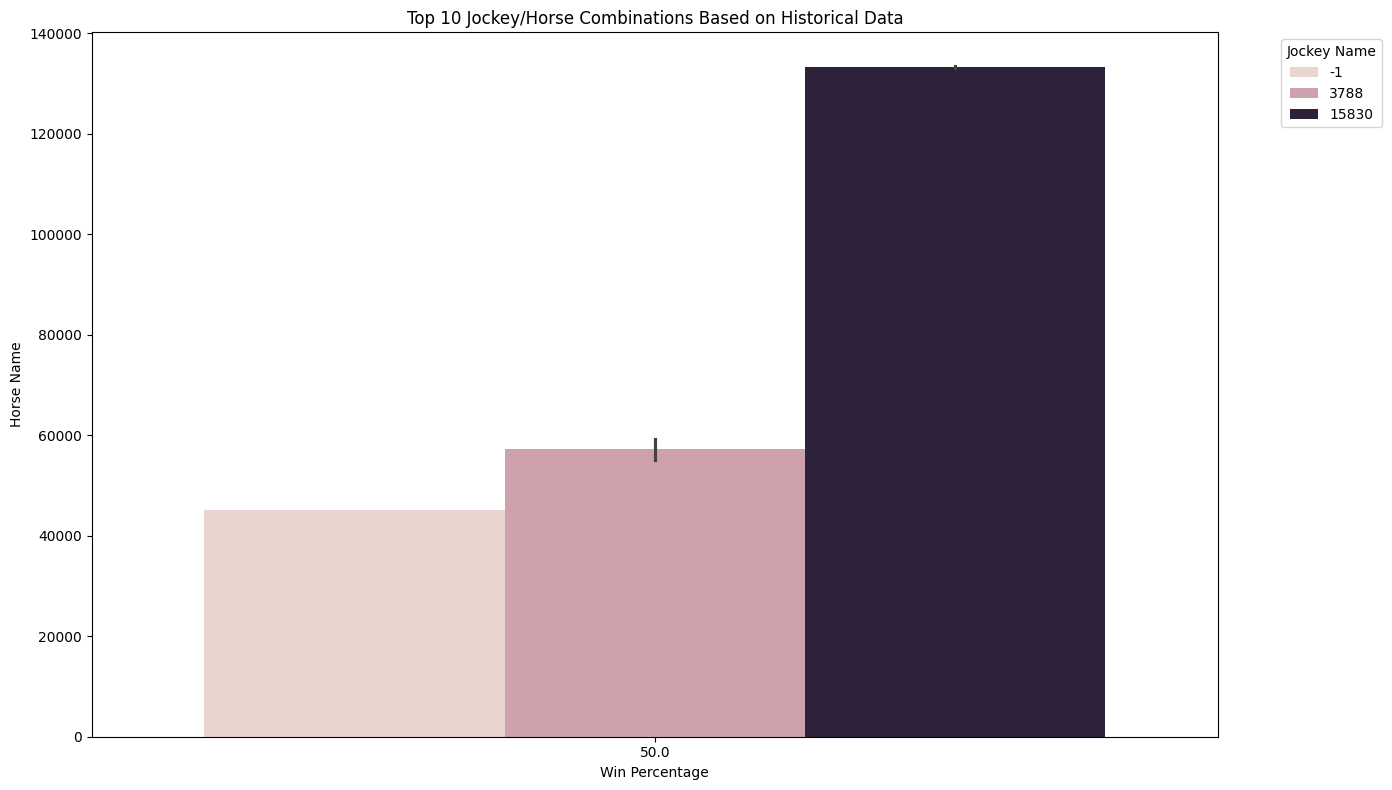
\includegraphics[width=0.8\textwidth]{images/top_jockey_horse_combinations.png} % Ensure this matches your file name
    \caption{Top 10 Jockey/Horse Combinations Based on Historical Data}
    \label{fig:top_jockey_horse_combinations}
\end{figure}

% Explanation for Figure 14
The bar plot illustrates the top 10 jockey/horse combinations based on historical win percentage. Each bar represents a specific combination of jockey and horse, with the height of the bar indicating the win percentage. The legend differentiates between the jockeys involved in these top combinations. This visualization helps in identifying the most successful jockey/horse pairings, providing insights into which combinations have historically performed best. Such information is valuable for predictive modeling and betting strategies, as it highlights the consistent winners over time.

\section{Conclusion}
The comprehensive analysis presented through various visualizations provides a clear understanding of the dataset and the performance of different machine learning models applied to horse racing predictions. The distribution plots (Figures \ref{fig:data_summary} and \ref{fig:distribution_distances}) reveal the variety and commonality of race distances and average speeds, highlighting key patterns in the dataset that can influence model predictions. The pairwise relationships (Figure \ref{fig:pairwise_relationships}) emphasize the correlations between significant variables such as distance, winning time, and average speed, showcasing the complexity and interdependence of these features.

The benchmarking results for classification and regression models (Figures \ref{fig:classification_models} and \ref{fig:regression_models}) illustrate the comparative performance of different algorithms, with random forest models demonstrating strong predictive accuracy and robustness. The ROC curve (Figure \ref{fig:roc_curve}) and learning curves (Figure \ref{fig:learning_curves}) further validate the efficacy of the random forest classifier, confirming its ability to distinguish between winning and losing outcomes with high precision. The confusion matrix (Figure \ref{fig:confusion_matrix}) provides detailed insights into the classifier's performance, indicating minimal misclassifications.

The residuals plot (Figure \ref{fig:residuals}) and precision-recall curve (Figure \ref{fig:precision_recall_curve}) offer additional perspectives on model performance, highlighting areas for potential improvement. The feature correlation heatmap (Figure \ref{fig:feature_correlation_heatmap}) and feature importance chart (Figure \ref{fig:feature_importances}) underscore the critical variables influencing the predictions, such as position and race distance. Finally, the top jockey/horse combinations (Figure \ref{fig:top_jockey_horse_combinations}) showcase the historical success of certain pairings, providing valuable insights for future predictions.

Overall, these visualizations collectively demonstrate the strengths and limitations of various machine learning models in predicting horse racing outcomes. The insights gained from this analysis can guide future model development, feature selection, and strategic decision-making, ultimately enhancing the accuracy and reliability of predictions in the horse racing domain.

The comprehensive quantitative benchmarking of machine learning algorithms presented in this study underscores the critical role these models play in data-driven decision making. Through the analysis of horse race predictions, the study meticulously evaluated a diverse array of algorithms, including linear regression, logistic regression, random forests, neural networks, and more. The findings revealed the distinct strengths and limitations of each approach, highlighting the exceptional performance of random forest models in terms of predictive accuracy and robustness. Detailed visualizations provided insights into data distributions, feature correlations, model performance, and the significance of various predictors. This methodological framework not only validates the effectiveness of machine learning algorithms in handling complex datasets but also serves as a valuable guide for quantitative researchers aiming to apply these techniques in various domains. The critical analysis of model performance, coupled with feature importance assessments, offers actionable insights that can enhance predictive accuracy and inform strategic decisions, reinforcing the value of structured, quantitative research in advancing the field of machine learning.

\section*{Experimental Methodology}

This section provides a comprehensive description of the experimental methodology used in this study. The entire experiment was executed in a Google Colab environment with the default runtime, which includes a GPU, 12GB of RAM, and ample storage. The total computation time for the experiment was 2 hours, 3 minutes, and 48 seconds. The methodology comprises several crucial steps: data collection, preprocessing, model development, training, evaluation, iterative reshuffling, feature importance analysis, and final insights and predictions.

\subsection*{Data Collection}
The dataset used in this study was sourced from Kaggle, specifically the horse racing dataset. This dataset contains various attributes such as race distances, winning times, horse positions, prize money, jockey names, and horse names. The dataset was downloaded and extracted using the following commands:
\begin{verbatim}
if not os.path.exists('horse_racing_data'):
    os.system('kaggle datasets download -d hwaitt/horse-racing')
    os.system('unzip horse-racing.zip -d horse_racing_data')
\end{verbatim}
The extracted data comprised multiple CSV files, which were verified by listing the files in the directory to ensure successful extraction.

\subsection*{Data Preprocessing}
Data preprocessing is a critical step to ensure data quality and consistency. The preprocessing steps included verifying data extraction, handling missing values, and feature engineering. The data types for each column were specified to avoid mismatches, and missing values were handled by filling numerical data with the mean and categorical data with the mode. Duplicate columns were removed, and data types were made consistent.

\subsubsection*{Verifying Data Extraction}
The files in the extracted directory were listed to ensure the dataset was correctly downloaded and extracted:
\begin{verbatim}
logging.info("Listing files in 'horse_racing_data' directory:")
logging.info(os.listdir('horse_racing_data'))
\end{verbatim}

\subsubsection*{Handling Missing Values and Data Cleaning}
Data cleaning involved specifying the data types for each column, removing duplicate columns, and handling missing values:
\begin{verbatim}
dtype_spec_horses = {...}
dtype_spec_races = {...}

horse_data = load_data_chunked(horse_files, dtype_spec_horses)
race_data = load_data_chunked(race_files, dtype_spec_races)

def remove_duplicates(data):
    data = data.loc[:, ~data.columns.duplicated()]
    data = data.reset_index(drop=True)
    return data

horse_data = remove_duplicates(horse_data)
race_data = remove_duplicates(race_data)
\end{verbatim}

\subsubsection*{Feature Engineering}
Feature engineering involved creating new features such as converting race distances into furlongs and calculating average speed:
\begin{verbatim}
def convert_distance(dist):
    try:
        parts = dist.lower().replace('m', ' ').replace('f', '').split()
        if len(parts) == 2:
            miles, furlongs = map(float, parts)
        elif len(parts) == 1:
            if 'm' in dist:
                miles = float(parts[0])
                furlongs = 0
            else:
                miles = 0
                furlongs = float(parts[0])
        else:
            return float('nan')
        return miles * 8 + furlongs  # 1 mile = 8 furlongs
    except:
        return float('nan')

merged_data['distance'] = merged_data['distance'].apply(convert_distance)
merged_data['avg_speed'] = merged_data['distance'] / merged_data['winningTime']
\end{verbatim}

\subsection*{Exploratory Data Analysis (EDA)}
EDA involved visualizing and summarizing the data to uncover patterns and relationships. Distribution plots, pairwise relationship plots, and heatmaps for feature correlations were used to provide valuable insights:
\begin{verbatim}
plot_distribution(merged_data, 'distance', 'Distribution of Distances', 'Distance (furlongs)')
plot_distribution(merged_data, 'avg_speed', 'Distribution of Average Speeds', 'Average Speed (furlongs/second)')
plot_pairwise_relationship(merged_data[['distance', 'winningTime', 'avg_speed']], 'Pairwise Relationships in Merged Data')
\end{verbatim}

\subsection*{Model Development}
A diverse set of machine learning models were selected for both regression and classification tasks. These models included linear regression, logistic regression, random forest regressor and classifier, MLP regressor and classifier, XGBoost classifier, Naive Bayes, decision trees, KNN, and a TensorFlow neural network. The implementation involved importing the necessary libraries and defining the models with their respective configurations.

\subsection*{Model Training and Evaluation}
The selected models were trained on the training dataset and evaluated using cross-validation techniques. Performance metrics such as accuracy, ROC AUC score, precision-recall curves for classification, and mean squared error (MSE) for regression were calculated to compare and select the best-performing models:
\begin{verbatim}
def train_and_evaluate(model_name, model, X_train_scaled, X_test_scaled, y_train, y_test):
    if model_name == 'tensorflow_classifier':
        model.fit(X_train_scaled, y_train, epochs=50, batch_size=32, validation_split=0.2, verbose=0)
        y_pred = (model.predict(X_test_scaled) > 0.5).astype("int32")
        accuracy = accuracy_score(y_test, y_pred)
        roc_auc = roc_auc_score(y_test, model.predict(X_test_scaled))
        return model_name, {'accuracy': accuracy, 'roc_auc': roc_auc}
    elif 'classifier' in model_name:
        model.fit(X_train_scaled, y_train)
        y_pred = model.predict(X_test_scaled)
        accuracy = accuracy_score(y_test, y_pred)
        roc_auc = roc_auc_score(y_test, model.predict_proba(X_test_scaled)[:, 1])
        return model_name, {'accuracy': accuracy, 'roc_auc': roc_auc}
    else:
        model.fit(X_train_scaled, y_train)
        y_pred = model.predict(X_test_scaled)
        mse = mean_squared_error(y_test, y_pred)
        return model_name, {'mse': mse}

results = evaluate_models(X_train_scaled, X_test_scaled, y_win_prob_train, y_win_prob_test)
\end{verbatim}

\subsection*{Iteration and Reshuffling}
To ensure the stability and reliability of the models, multiple iterations were conducted with different random splits of the data. This iterative process validated the consistency of the model's performance across various subsets of the dataset:
\begin{verbatim}
for i in range(5):
    results = evaluate_models(X_train_scaled, X_test_scaled, y_win_prob_train, y_win_prob_test)
    all_results.append(results)
\end{verbatim}

\subsection*{Feature Importance Analysis}
Feature importance analysis using models like random forests and XGBoost provided insights into the key factors influencing horse race outcomes. This analysis helped interpret the model's decisions and understand the underlying relationships within the data:
\begin{verbatim}
importances = models['random_forest_classifier'].feature_importances_
indices = np.argsort(importances)[::-1]
feature_names = X.columns

plt.figure(figsize=(14, 10))
plt.title("Feature Importances")
plt.bar(range(X.shape[1]), importances[indices], align="center")
plt.xticks(range(X.shape[1]), feature_names[indices], rotation=90)
plt.xlim([-1, X.shape[1]])
plt.show()
\end{verbatim}

\subsection*{Final Insights and Predictions}
The final insights and predictions were derived from the analyzed data. Identifying the top jockey/horse combinations to bet on, based on historical data, provided actionable recommendations. The results were saved in a CSV file for further analysis or sharing with stakeholders:
\begin{verbatim}
top_combinations.to_csv('best_jockey_horse_combinations.csv', index=False)
\end{verbatim}

This comprehensive methodology ensured a thorough quantitative benchmarking of various machine learning algorithms in the context of horse race predictions. Each step was carefully designed to maximize the quality and reliability of the insights derived from the data, contributing to the overall robustness of the predictive models.

\section*{Author Contributions}

The author, AP, conceptualized the idea and framework for this study, sourced and curated the dataset from Kaggle, and meticulously preprocessed the data to ensure quality and reliability. AP was responsible for developing, implementing, and debugging the machine learning models, leveraging a comprehensive suite of algorithms including linear regression, logistic regression, random forests, neural networks, and others. Additionally, AP conducted the exploratory data analysis and visualizations to uncover underlying patterns and correlations within the data.

AP utilized the Google Colab environment with the default computational runtime, which included 12GB of RAM, to execute and evaluate the models. The total execution time for the experiments was 2 hours, 3 minutes, and 48 seconds. Furthermore, AP transcribed the experimental methodology and results into LaTeX, and iteratively refined the document with the assistance of ChatGPT-4o. 

Data were sourced and are available from (https://www.kaggle.com/datasets/hwaitt/horse-racing/data ) (Accessed on 24/06/2024 ) 

Code is available on (github link ) 
\end{document}


\end{document}


\end{document}
